\cotefile{1}
\scanpage{79}

\uline{Corollaire 4} Soit $u$ un op. de Fredholm d'un espace de Hilbert $E$. Alors

\[
\boxed{|\alpha_n(u)|\leq\alpha_n(\deleted{\unsure{\sqrt{u^*u}}}|u|\deleted{{}_{\unsure{2}}})}\tag*{(18)}
\]

(\deleted{En} d'autres termes) les coefficients du développement de Fredholm $\det(1+zu)$ sont majorés en valeur, terme à terme, par les coefficients du déterminant de Fredholm $\det(1+z\unsure{h|H|\lvert u\rvert})$ relatif à l'hermitien positif $h=\sqrt{\unsure{uu^*|u^*u}}$. On en conclut en effet

\uline{Corollaire 5} Dans les conditions précédentes, on a

\[
|\det(1+zu)|\leq\det(1+|z|h)\quad\deleted{\unsure{(\sqrt{u^*u})}}\tag*{(19)}
\]

\unsure{Prouvons|Montrons} (18). On a \inserted{en effet}, $|\alpha_nu|=|\mathrm{Tr}_n\,\hat u|\leq\|\hat u_n\|_1=\unsure{\mathcal U_n|\mathcal A_n|\alpha_n}(\sqrt{u^*u})$ (formule (16)).

\deleted{\uline{Théorème 2} Soit $u$ une \deleted{application}\inserted{op.} de Fredholm dans l'espace de Hilbert $H$. Alors la suite \inserted{$(\lambda_i)$} des valeurs propres de $u$ est sommable \deleted{\unsure{et}} \deleted{\unsure{(1)}} \deleted{\illegible{4}} \deleted{\unsure{valeurs de $u$}}, on a}

\[
\boxed{\deleted{\det(1+u)=\prod_i(1+\lambda_i)}}\tag*{\deleted{(20)}}
\]

\deleted{\uline{Corollaire 1} Le déterminant de Fredholm $\det(1+zu)$ de $u$ est une fonction entière de genre $0$\,;}

\[
\deleted{\det(1+zu)=\prod_i(1+z\lambda_i)}\tag*{\deleted{(22)}}
\]

\deleted{\inserted{Appliquant (21) à $zu$ au lieu de $u$, on trouve}}

% margin note written sideways
\margin{\deleted{Le corollaire 1 \unsure{ci-}\unsure{dessus} équivaut \deleted{\unsure{aux}}\inserted{à la} formule, (23) $\alpha_n(u)=\sum_{i_1<\cdots<i_n}\lambda_{i_1}\deleted{\unsure{(u)}}\ldots\lambda_{i_n}\deleted{\unsure{(u)}}$ dont le \unsure{plus intéressant|premier cas particulier} est (23) $\boxed{\mathrm{Tr}\,u=\sum\lambda_i(u)}$}}

\deleted{\uline{Démonstration} du th. 2. \deleted{\unsure{Nous prouvons}} \unsure{On prouve} d'abord le lemme (20) \unsure{sur les valeurs}, \unsure{nous bornant à} la formule (20) : soit un \unsure{op. et un autre}, \illegible{3} \unsure{propre}, soit \unsure{une projection} \illegible{2}, alors tout \unsure{revient} qu'il en est \unsure{ainsi}, et que \illegible{1} est \unsure{identique} dès que \deleted{\unsure{tout}} \unsure{la} \illegible{1} est \unsure{nulle}.}

% archive sheet number: 80
\scanpage{80}

\deleted{\deleted{\unsure{Prouvons|Réunissons}\,;} Il suffit de prouver que \deleted{\unsure{tout} \illegible{2} \unsure{possible} $\sum\unsure{(z_1+\cdots+z_n)}$ est \unsure{majoré} par $\|u\|_1$ \unsure{distinct}. Soit \unsure{à cet effet}} $x_1,\ldots,x_n$ des vecteurs propres lin. \deleted{\unsure{à des valeurs propres}} indépendants associés aux valeurs propres $z_i$, \deleted{\unsure{soit}} on a $\sum|z_i|\leq\|u\|_1$. Soit en effet}

% margin note written sideways
\margin{\deleted{Nous prouvons au N° suivant que $\sum|\lambda_i|\leq\|u\|_1$. Ici, nous nous bornons à établir, plus élémentairement et \deleted{\unsure{par}} une proposition \unsure{pourtant plus faible},}}

\deleted{\deleted{\unsure{soit}} $p$ l'opérateur de projection orthogonale de $E$ sur le sous espace engendré par les $x_i$, on a}

\[
\deleted{|z_1+\cdots+z_n|=|\mathrm{Tr}\,pu|\leq\|pu\|_1\leq\|p\|\,\|u\|_1=\|u\|_1.}
\]

\deleted{\deleted{Comme} Les \deleted{\unsure{zéros}} inverses des zéros de $\det(1-zu)$ sont les $z_i$, et forment donc une suite sommable, que d'autre part les coefficients de $\det(1-zu)$ sont majorés, terme à terme, en valeur, par ceux de $\det(1+zh)$ où $h=\sqrt{u^*u}$ (prop. 1 corollaire 4). Nous supposons connu qu'une fonction entière dont les inverses des zéros forment une suite sommable, et \deleted{\unsure{que}} dont les coefficients sont majorés en module par ceux d'une série entière de genre 0, est elle \unsure{=|même} de genre 0. \deleted{\unsure{Ceci étant}, Prouvons} Il reste \deleted{\unsure{donc}}\inserted{donc} seulement à montrer que $\det(1+zh)$ est de genre 0.}

\deleted{\deleted{\unsure{Commençons} \inserted{donc} à vérifier les formules (23) pour $u=h$ \unsure{hermitien} $\geq0$, \unsure{les valeurs propres} \illegible{1} positives. Mais \deleted{\unsure{ce sont alors}} l'identité (22) signifie que $(\unsure{3|23|22})$ $\alpha_n(u)=\sum_{i_1<\cdots<i_n}\lambda_{i_1}\ldots\lambda_{i_n}$, ce qui se vérifie en effet immédiatement sur l'expression}}

\deleted{On aura $u=\sum\lambda_i\bar e_i\otimes e_i$ (où $(e_i)$ est un système orthonormal), d'où \deleted{\unsure{En effet, on aura}}\deleted{\unsure{déjà|donc}}}

\[
\deleted{\alpha_n(u)=\sum_{i_1,\ldots,i_n}\deleted{\unsure{\alpha_n(z_1e_1,\ldots)|\alpha_n(z_i e,\ldots)}}z_{i_1}\cdots z_{i_n}\,\alpha_n(\bar e_{i_1}\otimes e_{i_1},\ldots,\bar e_{i_n}\otimes e_{i_n}).}
\]

\deleted{\deleted{\unsure{et}} \deleted{\unsure{et}} $\alpha_n(\bar e_{i_1}\otimes e_{i_1},\ldots,\bar e_{i_n}\otimes e_{i_n})$ \deleted{\unsure{est}} est nul, sauf quand $i_1,\ldots,i_n$ sont distincts, auquel cas c'est égal à $\frac1{n!}$\,; rassemblant dans la somme les termes pour lesquels les $i_1,\ldots,i_n$ ne diffèrent que par l'ordre, on trouve bien (23).}

% archive sheet number: 81
\scanpage{81}

$f$ fonction convexe sur l'ouvert convexe $U$,

\[
(x,y)\in G_f\iff x\in U\text{ et } y>f(x)
\]

Soit \deleted{\unsure{$x,y$|$x_i,y_i$}} $(a,b)$ avec $b=f(a)$ $(a\in U)$, \deleted{\unsure{on|donc}} soit $H$ un hyperplan passant par $(a,b)$ ne rencontrant pas l'ouvert $G_f$, alors : 1) il est de la forme

\[
y-b=\deleted{\unsure{\sum c_i x_i+\beta}}=\sum c_i(x_i-a_i)
\]

(car ne \unsure{contient} pas la droite $x=a$), soit $y=L_a(x)$

2) On a $f(x)\geq L(x)$ pour \uline{\unsure{tout}} $x\in U$ (en effet, l'un des deux \deleted{\unsure{hyperplans}} $\frac12$ espaces \inserted{ouverts} déterminés par $H$ contient $G_f$, et ce ne peut être que celui donné par $y>L(x)$. \deleted{\unsure{donc}} d'où la conclusion).

3) On a pour $x\in E$ $f(x)=\sup_a L_a(x)$ (le sup étant obtenu), et réciproquement.

4) Si au point $a$, $f(x)$ est croissante alors les $c_i$ sont $\geq0$. En effet, si on avait p. ex $c_1<0$, alors $f(x_1,a_2,\ldots a_n)$ est croissante au point $x_1=a_1$,

\figure{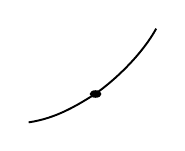
\begin{tikzpicture}[x=1cm,y=1cm]\draw[line width=.7pt] (0,0) .. controls (.35,.05) and (.62,.22) .. (.83,.35) .. controls (1.12,.55) and (1.45,.88) .. (1.62,1.19);\fill (.85,.36) ellipse (.075 and .048);\end{tikzpicture}}

et \deleted{de} minorée par $L(x_1,a_2,\ldots a_n)$, fonction linéaire prenant au point $a$ la même valeur que $f$. Cette dernière ne peut être strictement décroissante car on aurait $f(x_1)\leq f(a)\leq\unsure{\underline{f}|L|f}(x_1)$ pour $x_1<a_1$ voisin de $a_1$.

% archive sheet number: 82
\scanpage{82}

§. \uline{Inégalités de convexité et degrés remarquables d'opérateurs compacts}

\deleted{\unsure{La méthode de convexité}} \inserted{\textcircled{\scriptsize Th. 1}} \textcircled{1°} \deleted{\uline{Lemme fondamental}} \inserted{(H. Weyl).} Considérons deux suites finies

$(\alpha_i)_{1\leq i\leq n}$ et $(\beta_i)_{\unsure{1\leq i\leq n|i\leq n}}$ de nbres réels \inserted{on suppose} \deleted{la deuxième \illegible{1} \unsure{décroissante}}

\[
\boxed{\alpha_1\geq\alpha_2\ldots\geq\alpha_n}\quad\text{et}\quad
\boxed{\alpha_1+\cdots+\alpha_{\unsure{M|N|m}}\leq\beta_1+\cdots+\beta_M\enspace\text{pour }M=1,\ldots n.}\tag*{(1)\quad(2)}
\]

Soit $\varphi(t_1,\ldots,t_n)$ une fonction numérique \uline{convexe} et \uline{symétrique} sur $R^n$. On suppose vérifiée l'une des deux conditions suivantes : a) $\varphi$ est croissante \deleted{\unsure{(pour}}\inserted{en} chaque argument $t_i$ \deleted{la restriction d'un ensemble sur $R^n$} b) $\sum_{i=1}^n\alpha_i=\sum_{i=1}^{n}\beta_i$.

% slanted
\margin{\unsure{fonction} où l'on \unsure{devrait} \unsure{admettre} \unsure{H} \illegible{1} \deleted{\unsure{partie}} \unsure{un} convexe ouvert.}

Sous ces conditions, on a

\[
\varphi(\alpha_1,\ldots,\alpha_n)\leq\varphi(\beta_1,\ldots\beta_n)\tag*{(3)}
\]

\deleted{Appliquons \unsure{tout de suite} le corollaire suivant, qui \unsure{seul nous} \illegible{1} \unsure{pour la} \unsure{question} qui \unsure{effacerait} \illegible{1}. On en conclut immédiatement le}

\deleted{\uline{Corollaire 1}} \inserted{\textcircled{2°}} Soit $f(\rho_1,\ldots,\rho_n)$ fonction \deleted{\unsure{continue|numérique}} \inserted{\uline{numérique symétrique}} de $n$ arguments \deleted{\unsure{positifs}} \inserted{$\rho_i>0$}, telle que $f(e^{t_1},\ldots,e^{t_n})$ soit une fonction \uline{convexe} de $(t_1,\ldots t_n)\in R^n$. Soient $(\rho_1,\ldots\rho_n)$ et $(\sigma_1,\ldots,\sigma_n)$ deux suites \inserted{finies} positives, telles que \deleted{\unsure{(Hies.)}} \textcircled{4} $\boxed{\rho_1\geq\rho_2\ldots\geq\rho_n}$ et que \deleted{\unsure{\ensuremath{\sum\rho_i}}} \textcircled{5} $\boxed{\rho_1\cdots\rho_M\leq\sigma_1\cdots\sigma_M}$ pour \deleted{tout} $M=1,\ldots n$. On suppose vérifiée l'une des deux conditions suivantes :

% slanted
\margin{Il suffit que l'ensemble où est définie $f$ soit une partie \unsure{logarithmiquement} \unsure{convexe} \unsure{convenable} et symétrique.}

a) $f$ est \inserted{définie et continue pour $\rho_i\geq0$, et} fonction croissante \deleted{des} \deleted{\unsure{chacun des|chaque argument $\rho_i$}}\inserted{de chaque argument} $\rho_i$ b) $\rho_1\cdots\rho_n=\sigma_1\cdots\sigma_n\ne0$. Sous ces conditions, on a

\[
f(\rho_1,\ldots\rho_n)\leq f(\sigma_1,\ldots\sigma_n)\tag*{\deleted{\unsure{(4)}} (6)}
\]

En effet, si les $\rho_i,\sigma_i$ sont $>0$, cet énoncé est manifestement équivalent à l'énoncé du \deleted{lemme}\inserted{th.}, en posant $\alpha_i=\log\rho_i$, $\beta_i=\log\sigma_i$. \inserted{Cela prouve le \deleted{\unsure{corollaire}}\inserted{(2°)} en particulier dans le cas b).}

\deleted{\unsure{On en conclut}, puisque} \inserted{Montrons que} dans le cas a), tout \deleted{l'un et des} systèmes $(\rho_i),(\sigma_i)$ tels que $\rho_i\geq0$, $\deleted{\unsure{\sigma_i\geq0|\rho_i>0}}$ \inserted{$\rho_1\geq\rho_2\ldots\geq\rho_n\geq0$,} $\rho_1\cdots\rho_M\leq\sigma_1\cdots\sigma_M$ pour $M=1,\ldots n$, \deleted{\unsure{et naturellement} $\rho_1\ldots\rho_n=\sigma_1\ldots\sigma_n$)} \deleted{\unsure{et l'adhérence}} \inserted{est limite dans $R^{2n}$} \deleted{\unsure{de sa partie formée des systèmes tels}} \inserted{de systèmes analogues} $(\rho'_i,\sigma'_i)$ avec $\rho'_i>0$, $\sigma'_i>0$ (d'où résultera le \deleted{corollaire}\inserted{(2°) dans le cas a)} par prolongement par continuité). En effet, si \deleted{\unsure{les $\rho_i$}} \inserted{$\sigma_i>0$ pour tout $i$,} on voit qu'en \deleted{\unsure{tous les cas}} augmentant \inserted{de suffisamment peu} les $\rho_i$ qui seraient nuls, \deleted{\unsure{sont nuls, et il suffit de reprendre les inégalités pour|et il suffit d'approcher les systèmes}} on satisfait encore aux conditions imposées, \deleted{\unsure{et si} les systèmes $(\rho'_i)$ et $(\sigma'_i)$, avec $\rho'_i=\sigma'_i=\frac1n$ pour tout $i$. D'autre part} d'où la conclusion dans ce cas.

\margin{\unsure{?}}

\deleted{Si plus généralement, \unsure{dans|donc} \illegible{1} \unsure{l'on} \illegible{2} \unsure{qui sont} \illegible{1} d'abord \illegible{1}}

% archive sheet number: 83
\scanpage{83}

\deleted{approcher $(\rho_i)(\sigma_i)$ par les systèmes $(\rho'_i)=(\rho_i)$, $(\sigma_i+\varepsilon)$ \inserted{$\unsure{\sigma'_i}$} \illegible{1} du \unsure{même} \illegible{1} \unsure{pour} $k=\unsure{n}$, $\rho'_i,\sigma'_i$ qui satisfont encore aux conditions \unsure{énumérées} \unsure{sauf} que $\sigma'_{n-1}\ne0$ (en posant}

Il suffit donc, dans le cas \deleted{\unsure{général}}\inserted{$\sigma_n=0$}, \deleted{d'\unsure{associer|approcher}} \inserted{d'approcher} $(\rho_i)$ $(\sigma_i)$ par des \inserted{systèmes admissibles} $(\rho'_i),(\sigma'_i)$ avec $\sigma_n>0$, et on prendra

\deleted{\deleted{\unsure{évidemment}} \unsure{supposons} par des $(\rho'_i),(\sigma'_i)$, avec $\sigma'_{n-1}>0$, comme on voit en posant $(\rho'_i)=(\rho_i)$, $\sigma_i=\sigma'_i+\varepsilon$ pour \deleted{tout} $i\leq n-1$, $\sigma'_n=\sigma_n$ (on aura un système admissible, en particulier $\prod\rho'_i=\prod\sigma'_i=0$), ce qui nous ramène au cas où $\deleted{\unsure{\sigma'}}\sigma_{n-1}>0$, $\sigma_n=0$. \deleted{\unsure{et dont}}}

\deleted{Dans ce cas, si on pose $\sigma'_i=\sigma_i$ pour $i\leq n-1$, $\sigma'_n=\sigma_n+\varepsilon$, le système $(\rho_i),(\sigma'_i)$ est admissible \inserted{pour $\varepsilon$ assez petit}, sauf que, dans le cas où on impose $\prod\rho_i=\prod\sigma_i$, on n'aura \deleted{\unsure{peut-être}} pas $\prod\rho_i=\prod\sigma'_i$. Mais en augmentant suffisamment peu les $\rho_i$ nuls, on obtient un système $(\rho'_i)$ tel qu'on ait encore \deleted{\unsure{et $\rho$}} $\rho'_1\ldots\rho'_q\leq\sigma'_1\ldots\sigma'_q$ pour $q=1,\ldots n$, et \deleted{\unsure{même}}\inserted{par} augmentation éventuelle de $\rho'_n$ \deleted{\unsure{jusqu'à}}\inserted{$\rho''_n$}, \deleted{on obtient $\rho'_1\ldots\rho'_{n-1}\rho''_n=\sigma'_1\ldots\sigma'_n$. Ce système $\rho'_n=$}}

simplement $\rho'_i=\rho_i$, $\sigma'_i=\sigma_i+\varepsilon$.

Prouvons maintenant le lemme. Il est bien connu qu'une \deleted{toute} fonction convexe \deleted{\unsure{$f$}} $\varphi$ sur $R^n$ est de la forme $\varphi=\sup_{k\in\unsure{K}}L_k$ où les $L_k$ sont des \deleted{\unsure{formes}}\inserted{fonctions} \uline{linéaires} \inserted{affines} sur $R^n$ (car résulte du fait que la partie de $R^n\times R$ au dessus du graphe de $\varphi$ est convexe $\div$ par définition des fonctions convexes et fermée car $\varphi$ est continue, et donc intersection de demi-espaces fermés, dont on constate aussitôt qu'ils \deleted{\unsure{ne peuvent} \unsure{avoir} pour} \inserted{peuvent} se mettre sous la forme \inserted{d'équations} $L_k(t)\geq0$).

De plus, si $\varphi$ est croissante, on voit \deleted{\unsure{qu'on} \illegible{2}}\inserted{que} les $L_k$ \unsure{croissantes|le sont}, i.e. \deleted{à coefficients} de la forme $L_k(t)=\sum_{i=1}^n a_it_i+\unsure{h|b|b_k}$, \deleted{\unsure{où les}}\inserted{avec} $a_i\geq0$ pour \deleted{tout} $i$. \deleted{Pour le voir,} : En effet, si on avait $a_i<0$, alors \deleted{la fonction} on

% archive sheet number: 84
\scanpage{84}

fixant les arguments $t_j$ pour $j\ne i$, $L_k(t)=L_k(t_1,\ldots t_n)$ \deleted{serait une fonction linéaire strictement décroissante de \deleted{\unsure{$t_i$}} $s=t_i$, majorée par la fonction continue croissante $\inserted{\varphi(t)=}\varphi(t_1,\ldots,t_n)$, \deleted{\unsure{donc}} ce qui est manifestement impossible, \deleted{\unsure{puisque}} car \unsure{$L$|$\lambda$}$(s)\to\infty$ si $s\to-\infty$, et que $\varphi(s)$ reste borné pour $s\to-\infty$.}

on aurait $L(t)\to\unsure{0|\infty}$ si $t_i\to-\infty$, tandis que $\varphi(t)$ \deleted{\unsure{restant|resterait}}\inserted{resterait} borné pour $t_i\to-\infty$, ce \deleted{\unsure{(en effet)}} qui est incompatible avec $L(t)\leq\varphi(t)$ pour \deleted{tout} $t$. \deleted{\unsure{$f$}} Comme \deleted{\unsure{maintenant}}\inserted{enfin} $\varphi$ est aussi supposée symétrique, $L\deleted{\unsure{(t_1,\ldots,t_n)}}\leq\varphi\deleted{\unsure{(t_1,\ldots,t_n)}}$ \inserted{($L$ fonction sur $R^n$)} implique $\deleted{\unsure{L_k(t_{\sigma1},\ldots,t_{\sigma n})\leq\varphi(t_{\sigma1},\ldots,t_{\sigma n})}}\inserted{\sigma L\leq\varphi}$ pour \deleted{tout} $\sigma\in\unsure{\mathscr S_n|\mathfrak S_n}$ (groupe des permutations des $n$ premiers entiers, i.e. \inserted{avec $\sigma L(t_1,\ldots t_n)=L(t_{\sigma^{-1}1},\ldots t_{\sigma^{-1}n})$}), donc on aura aussi

\[
\deleted{\unsure{\varphi(t_1,\ldots,t_n)|\varphi(t)}}\varphi=\sup_k\sup_{\sigma\in\mathscr S_n}\sigma.L_{k}\deleted{\unsure{(t_1,\ldots,t_n)}}\tag*{(7)}
\]

Il s'ensuit que \deleted{\unsure{si}} pour prouver (\unsure{1|3}), il suffit de prouver que \inserted{pour $L=L_k$, on a} \deleted{$\sigma L_k\deleted{\unsure{(\alpha_{\sigma1})}}(\alpha_1,\ldots\alpha_n)\leq\varphi(\beta_1,\ldots\beta_n)$ pour tout $k$, et tout $\sigma\in\mathscr S_n$. \unsure{Remplaçant} \deleted{\unsure{Désignant}} \unsure{enfin|alors} $\sigma L_k$ par $L$, on est ramené à prouver}

\[
\sup_{\sigma\in\mathscr S_n}(\sigma.L)(\alpha_1,\ldots\alpha_n)\leq\sup_{\sigma\in\mathscr S_n}(\unsure{\sigma|\tau}L)(\beta_{\unsure{\sigma1}},\ldots\beta_{\unsure{\sigma n}})\tag*{(8)}
\]

(car le deuxième mb en effet est $\leq\varphi(\beta_1,\ldots\beta_n)$) \deleted{\unsure{Pour le|Dans}}\inserted{Dans cette} inégalité, \deleted{\unsure{$L$ est une forme linéaire}} $L(t_1,\ldots t_n)=\sum_i^n a_it_i+b$, \deleted{\unsure{affine et}} avec des \deleted{\unsure{$a_i$}} coefficients quelconques dans le cas b), et des $a_i>0$ pour tout $i$ dans le cas a) du lemme. \deleted{\unsure{Désignons} \unsure{Remarquons},} On peut évidemment \deleted{\unsure{retrancher des deux membres} \unsure{l'effet de} \illegible{2}} supposer $b=0$.

\deleted{D'après un lemme connu, Il suffit \deleted{$\sum a_i b_i$} $L(\alpha_1,\ldots,\alpha_n)\leq L(\unsure{\beta_1,\ldots})$ \unsure{Notons que|lorsque} $\sum a_i\alpha_i\leq\sum a_i\alpha_{\sigma i}$ quand $\sigma$ est une permutation telle que la suite des $a_{\sigma i}$ est \uline{décroissante}, ce qui}

D'après un lemme connu, \inserted{valable du fait que $\alpha_1\geq\alpha_2\geq\ldots\geq\alpha_n$,} la somme $\sum a_{\sigma i}\alpha_i\inserted{=\sum a_i\alpha_{\sigma^{-1}i}}$ est maximum, pour $\sigma\in\mathscr S_n$ variable,

% archive sheet number: 85
\scanpage{85}

quand la suite $(a_{\sigma i})$ est décroissante, on est donc \deleted{\unsure{en réarrangeant au besoin les indices|on peut donc se ramener au besoin}} \deleted{\unsure{supposer, pour prouver (8), que la suite} $a_1\geq a_2\ldots\geq a_n$} ramené à prouver que si $a_1\geq a_2\ldots\geq a_n$, on a $\sum a_i\alpha_i\leq\deleted{\unsure{a_i\alpha|\sum a_i\alpha_i}}\sum a_i\beta_i\deleted{\unsure{\sum a_i\alpha|\sum a_i\alpha_i}}$, \deleted{\unsure{en supposant ou que}}\inserted{pourvu que} les $a_i$ soient positifs \deleted{si on n'est pas dans le cas b) du lemme} ou qu'on ait $\sum\alpha_i=\sum\beta_i$. Or on a en effet

\[
\begin{aligned}
\sum a_i\alpha_i={}&(a_1-a_2)\alpha_1+(a_2-a_3)(\alpha_1+\alpha_2)+\cdots+(a_{n-1}-a_n)(\alpha_1+\cdots+\alpha_{n-1})\\
&+a_n(\alpha_1+\cdots+\alpha_n)
\end{aligned}\tag*{(9)}
\]

\deleted{\unsure{et on a}} et une formule analogue pour $\deleted{\unsure{\sum a_i\alpha_i}}\sum a_i\beta_i$. Comme les coefficients $(a_1-a_2),\ldots,(a_i-a_{i\unsure{-1|+1}}),\ldots(a_{n-1}-a_n)$ sont positifs, \deleted{\unsure{on conclut que la somme relative|ainsi que}} et que $\deleted{\unsure{\sum}}\alpha_1\leq\beta_1,\ldots(\alpha_1+\cdots+\alpha_{n-1})\leq(\beta_1+\cdots+\beta_{n-1})$, on en conclut que tous les termes de la somme relative aux $\alpha_i$ sont majorés par les termes correspondants de la somme relative aux $\beta_i$, à l'exception \inserted{à priori} du dernier. Mais on a aussi $a_n(\alpha_1\unsure{+\cdots+|\ldots}\alpha_n)\leq a_n(\beta_1+\cdots+\beta_n)$ dans \deleted{\unsure{du terme du dernier}}\inserted{le cas a)} du lemme ($a_n\geq0$, $\sum\alpha_i\leq\sum\beta_i$) et dans le cas b) ($\sum\alpha_i=\sum\beta_i$), d'où \deleted{la conclusion}\inserted{l'inégalité (1)}.

\deleted{\unsure{Notons}} Signalons en passant le

% slanted
\margin{\uline{petits caractères}}

\uline{Corollaire \unsure{bis|1bis|1a}} Sous les conditions de \deleted{la prop. \unsure{du} corollaire 1, b,} \inserted{th. 1, 2°, b)} \deleted{\unsure{(hypothèse du corollaire 1, et|(resp. du corollaire 1, a))} \unsure{la prop. corollaire, b)|les mêmes hypothèses}} on aura aussi, \deleted{\unsure{si on a pour tout} \unsure{$\sigma$}}

\[
f\left(\frac1{\sigma_1},\ldots\frac1{\sigma_n}\right)\leq f\left(\frac1{\rho_1},\ldots,\frac1{\rho_n}\right)\tag*{(10)}
\]

En effet, de $\rho_1\ldots\rho_n=\sigma_1\ldots\sigma_n$ on tire pour tout \inserted{$1\leq\unsure{M|N}\leq n$ :}

\[
\rho_M\rho_{M+1}\ldots\rho_n=\frac{\sigma_1\ldots\sigma_{M-1}}{\rho_1\ldots\rho_{M-1}}\sigma_M\ldots\sigma_n,\qquad\text{d'où }\rho_M\ldots\rho_n\leq\sigma_M\ldots\sigma_n
\]

en vertu de $\sigma_1\ldots\sigma_{M-1}\leq\rho_1\ldots\rho_{M-1}$. Il s'ensuit que que les suites $(\frac1{\rho_n},\ldots\frac1{\rho_1})$ et $(\unsure{(}\frac1{\sigma_n},\ldots\frac1{\sigma_1})$ satisfont encore aux conditions du corollaire (la première étant décroissante, les produits \deleted{\unsure{qui interviennent par}} des $\frac1{\rho_i}$ ég. au produit des $\frac1{\sigma_i}$, et enfin $\frac1{\rho_n}\ldots\frac1{\rho_i}\leq\frac1{\sigma_n}\ldots\frac1{\sigma_i}$ pour $1\leq M\leq n$), d'où l'inégalité (10).

% archive sheet number: 86
\scanpage{86}

\margin{\inserted{Bien entendu, en remplaçant au besoin $\varphi$ par \deleted{\unsure{$f$}} son symétrique,}}\unsure{En th. 1, 1°, hypothèse b)}

\deleted{Bien entendu, \unsure{en vertu de} l'inégalité \unsure{indiquée|analogue}, $(4)$ $\sum\varphi(-\alpha_1,\ldots,-\alpha_n)\leq\sum\varphi(-\beta_1,\ldots,-\beta_n)$}

\uline{Remarque 1} Notons \deleted{\unsure{d'ailleurs|toutefois}} que si deux suites $(\alpha_i)_{i\leq n},(\beta_i)_{i\leq n}$ satisfont aux conditions générales du \deleted{lemme}\inserted{th. 1, 1°} \inserted{$(\alpha_1\geq\ldots\geq\alpha_n,\ \alpha_1+\cdots+\alpha_{\unsure{M|N|m}}\leq\beta_1+\cdots+\beta_M\ \deleted{\unsure{et}}\ 1\leq M\leq n$} alors \deleted{il en est de les \unsure{mêmes suites} $(\alpha_i)_{i\leq p},(\beta_i)_{i\leq p}$ pour tout $1\leq p\leq n$, \unsure{(ceci pour $p=n$ bien que} $\sum_1^p\alpha_i=\sum_1^p\beta_i$), donc on peut leur appliquer la \unsure{formule} du lemme, et en particulier par exemple $\varphi(\alpha_1,\ldots,\alpha_p)$ qu'on obtient en remplaçant $\alpha_{p+1},\ldots,\alpha_n$ et $\beta_{p+1},\ldots,\beta_n$ par}

\inserted{les suites à $k$ éléments} $(\alpha_i)_{i\leq k}$ et $(\beta_i)_{i\leq k}$ \inserted{satisfont aux conditions analogues} \deleted{quelque que soit}\inserted{quel que soit} $1\leq k\leq n$. On peut donc appliquer à ces suites le même lemme, et on trouve \deleted{\unsure{donc}}\inserted{p. ex.} que \deleted{\unsure{(quitte à} \illegible{2} \unsure{le lemme}} \inserted{si $\varphi$ est une fonction convexe} croissante de \uline{$k$} arguments, on a aussi $\varphi(\alpha_1,\ldots\alpha_k)\leq\varphi(\beta_1,\ldots,\beta_k)$. La remarque analogue vaut pour les \deleted{corollaire 1 du lemme}\inserted{conditions du th. 1, 2°}.

% slanted
\margin{\uline{Remarque 2} Si on suppose $(\alpha_i)$ $(\beta_i)$ \unsure{comme} dans l'\unsure{exposé a|espace}, et que $f(\alpha_1\ldots\alpha_n)\leq f(\beta_1\ldots\beta_n)$ pour \deleted{\unsure{toute}} $f$ telle \unsure{que} \ldots{} alors on a $\sum_1^m\alpha_i\leq\sum_1^m\beta_i$ (évidemment, cela revenant à $\sup_H\sum_{i\in H}\alpha_i$, \deleted{\unsure{où}} $H$ à \deleted{\unsure{au plus}} $m$ éléments)}

\deleted{\uline{Réciproque et exemples de convexité du corollaire 1.}}

Donnons maintenant des cas intéressants de fonctions $f$ satisfaisant aux conditions du \deleted{corollaire 1}\inserted{th. 1, 2°}. \deleted{\unsure{qui est}}

Si \uline{\deleted{\unsure{$f(\rho_1$}} $f(\rho_1,\ldots\rho_n)$ est une fonction convexe} croissante des \inserted{l'ens. des} arguments $\rho_i\geq0$, alors $f(e^{t_1},\ldots,e^{t_n})$ est \deleted{\unsure{convexe}}\inserted{une} fonction convexe de \deleted{\unsure{chacun des arguments}} $(t_i)\in R^{n}$. Comme \deleted{la fonction convexe $f$ \unsure{sera celle qui est}} \inserted{$f$ sera} une enveloppe supérieure de fonctions \deleted{\unsure{linéaires}}\inserted{linéaires} affines $\inserted{\sum a_i x_i+b}$ \inserted{avec la propriété $a_i\geq0$ (!)}, $f(e^{t_1},\ldots,e^{t_n})$ sera enveloppe supérieure \deleted{et que toute fonction convexe} de fonctions $\sum a_i e^{t_i}+b$, qui sont convexes (car \deleted{\unsure{si}} les fonctions $e^{t_i}$ sont convexes, et les $a_i$ positifs), donc elle sera elle-même convexe.

En particulier, \deleted{si $f$ par une norme \deleted{fonction} de la. Un} \unsure{appelons|appl.ons}, \uline{normes de Schatten} sur $R^n$ toute \uline{norme} $N(x)=N(x_1,\ldots x_n)$ qui est symétrique, telle que $N(x_1,\ldots x_n)=N(|x_1|,\ldots|x_n|)$, \deleted{et qui est fonction croissante de chacun des arguments pour} \inserted{$x_1\geq0,\ldots x_n\geq0$}, \deleted{\unsure{et par le fait est donc} \illegible{2}} \inserted{normalisée par $N(e_1)=1$.}

% margin note written sideways
\margin{Alors on prouve que $N$ est fonction croissante \deleted{\unsure{des arguments}} \unsure{(ens)} des \unsure{longueurs} des éléments positifs ((car la boule unité, étant stable par multiplication par une \unsure{homothétie|fonction} $(\lambda_i)$ avec $|\lambda_i|=1$ pour \deleted{tout} $i$, le sera pour \deleted{\unsure{toute}} fonction majorée par $1$ en module).}

% archive sheet number: 87
\scanpage{87}

\uline{norme de Schatten} $N(x_1,\ldots x_n)$ satisfait \deleted{à la condition envisagée}\inserted{à l'hypothèse} dans l'énoncé du \deleted{corollaire 1}\inserted{th. 1, 2°} \deleted{\unsure{p.p. la condition de la fonction|application suivante}}\inserted{pour la fonction $f$}. On en conclut, si $(\rho_i)$ \deleted{$\unsure{\rho_i|\rho(x)}$} et $(\sigma_i)$ sont comme dans le \unsure{th.}, :

% slanted
\margin{\textcircled{\unsure{11|13}} $N(\rho_1,\ldots\rho_n)\leq N(\sigma_1,\ldots,\sigma_n)$ et plus généralement, compte tenu d'une remarque qui précède, et en \deleted{\unsure{pour que}} posant pour $1\leq k\leq n$ : $N(\rho_1,\ldots\rho_k)=N(\rho_1,\ldots\rho_k,0,\ldots,0)$ \textcircled{12} $N(\rho_1,\ldots\rho_k)\leq N(\sigma_1,\ldots,\sigma_k)$ pour $1\leq k\leq n$}

\deleted{\unsure{De même}, si on sait que la fonction $(e^{t_i})^p$ étant une \unsure{fonction convexe}} \deleted{\uline{la fonction} $f(r_1,\ldots r_n)=r_1^p+\cdots+r_n^p$, $p$ est un nb réel \uline{quelconque}, satisfait aux \deleted{\unsure{conditions}} conditions \deleted{\unsure{du lemme}} envisagées dans le \uline{corollaire 1}, \deleted{\unsure{donc} dans l'hypothèse b, et même \deleted{\unsure{à toutes les}} conditions envisagées dans l'hypothèse a.}}

Par suite, \deleted{\unsure{on a} \illegible{1} \unsure{inégalités}}\inserted{sous les conditions} de l'hypothèse b, \deleted{\unsure{on}} $(\prod_1^{\unsure{M|N|m}}\rho_i\leq\prod_1^M\sigma_i\ \inserted{(\text{pour }1\leq M\leq n)},\ \prod_1^n\rho_i=\prod_1^n\sigma_i\ne0)$ on aura

\[
\sum_1^n\rho_i^p\leq\sum_1^n\sigma_i^p\qquad(p\text{ réel.})\tag*{(15)}
\]

\deleted{\unsure{et sous les cond}} \inserted{et si $p\geq0$,} on aura, pourvu que $\prod_1^M\rho_i\leq\prod_1^M\sigma_i$ pour \inserted{$1\leq M\leq n$}, \deleted{on aura}

\[
\sum_1^k\rho_i^p\leq\sum_1^k\sigma_i^p\qquad(p\geq0,\ \deleted{\unsure{et}} k=1,\ldots n.)\tag*{\deleted{\unsure{(12)}}\inserted{(16)}}
\]

\deleted{Remarquons d'ailleurs que de ce que $(\rho_i),(\sigma_i)$, \deleted{\unsure{positifs}}\inserted{positifs} \unsure{donnés}, \deleted{\unsure{dès}} satisfaisant aux inégalités (16) pour \deleted{tout} $k$, et \deleted{tout} $p$ entier $\geq0$, on peut \deleted{\unsure{en conclure}}\inserted{réciproquement}}

\deleted{\unsure{Nous pouvons arriver à}} \uline{Th 2} (\uline{Premier Théorème de convexité dans les espaces de Hilbert})

\deleted{\unsure{1)}} Soit $u$ un opérateur compact dans un espace de Hilbert, soit \deleted{\unsure{$\varphi$ la suite}} $f$\inserted{$(r_1,\ldots r_n)$} une fonction \inserted{continue et symétrique} de $n$ arguments $r_i\geq0$, croissante par r. à chaque $r_i$, et telle que $f(e^{t_1},\ldots,e^{t_n})$ soit fonction convexe de $(t_i)\in R^n$. Alors on a (\deleted{\unsure{en prenant} $\rho_i$} (avec les notations indiquées au N° \unsure{?|3}, avant la prop 3)

\[
f(|\lambda_1|,\ldots,|\lambda_n|)\leq f(\rho_1,\ldots\rho_n)\tag*{(17)}
\]

Il suffit en effet de conjuguer le corollaire 1 du lemme 1 \deleted{\unsure{(cas de}} (hypothèse a)) avec le N° \unsure{?|2}, prop 3, corollaire 2. -- En particulier

\uline{Corollaire 1} Si $f\deleted{\unsure{(r)|(\rho)}}$ est une fonction \deleted{\unsure{croissante|convexe}}\inserted{continue} croissante de $r\geq0$ telle que $f(e^t)$ soit convexe, et $u$ un op. compact dans un espace de Hilbert, on a

% archive sheet number: 88
\scanpage{88}

En \unsure{dernier|deuxième|troisième|anticipant} lieu, soit $f(\unsure{s|r|\rho})$ une fonction définie pour $s>0$, telle que $f(e^t)$ soit convexe, posons $f(s_1,\ldots,s_n)=\sum_1^n f(s_i)$, c'est une fonction symétrique des \deleted{\unsure{nombres}}\inserted{\unsure{argts|variables}} $s_i>0$, et telle que $f(e^{t_1},\ldots,e^{t_n})$ soit convexe. Par suite, \deleted{\unsure{$F$}} $f(s_1,\deleted{\unsure{+}}\ldots s_n)$ satisfait aux conditions du corollaire 1, sous l'hypothèse b. Si on suppose de plus $f(s)$ croissante, et définie et continue aussi pour $s\geq0$, alors $f(s_1,\ldots s_n)$ satisfait \unsure{même} aux conditions du \deleted{corollaire 1}\inserted{th. 1, 2°} sous l'hypothèse a.

D'où, \deleted{\unsure{avec la hypothèse}} \inserted{sous les conditions b,} \deleted{convenables sur $(\alpha_i),(\beta_i)$, \unsure{les inégalités}} l'inégalité

\[
\sum_1^n f(\rho_i)\leq\sum_1^n f(\sigma_i)\tag*{(13)}
\]

et sous les conditions de \unsure{b)|a)}, compte tenu d'une remarque précédente, la suite d'inégalités

\[
\sum_1^k f(\rho_i)\leq\sum_1^k f(\sigma_i)\qquad(k=1,\ldots n)\tag*{(14)}
\]

Prenons p.ex, \deleted{\unsure{$p$ positif et|pour}}\inserted{pour $p$ réel quelconque} $f(s)=s^p$, \inserted{$(s>0)$} on a alors $f(e^t)=e^{pt}$, qui est bien une fonction convexe. \deleted{\unsure{$f$ elle}}\inserted{$f(r)$} est définie et \deleted{\unsure{même}} continue pour $s\geq0$, et \deleted{\unsure{une}} fonction croissante de $s$, dès que $p\geq0$. \deleted{\unsure{On obtient donc}}

% archive sheet number: 89
\scanpage{89}

\[
\deleted{\unsure{f(\rho|f(\rho)}}\sum_1^{\unsure{k|n}}f(|\lambda_i|)\leq\sum_1^k f(\rho_i)\qquad\deleted{(k\leq\dim H)}\inserted{(k=1,\ldots)}\tag*{(18)}
\]

En particulier, \deleted{\unsure{pour que}} si \deleted{\unsure{$\dim$}} $\unsure{E|u}$ est de dimension infinie, si \inserted{la série} $\sum_{i=0}^{\infty}f(\rho_i)$ \deleted{\unsure{conv., alors|converge, alors}}\inserted{est convergente}, il en est de $=$ de $\sum_{\unsure{i|j}=0}^{\infty}f(|\lambda_i|)$, et on a

\[
\sum_{i=1}^{\infty}f(|\lambda_i|)\leq\sum_{i=0}^{\infty}f(\rho_i)\tag*{(19)}
\]

En particulier, faisant $f(\unsure{r|a})=r^p$ $(p>0)$, on trouve

\uline{Corollaire 2} Soit $u$ un op. compact dans un espace de Hilbert $E$, et soit $p>0$. Alors, pour tout entier $k>0$

\[
\boxed{\sum_{i=1}^k|\lambda_i|^p\leq\sum_{\unsure{j|i}=1}^k\rho_i^p\deleted{=\|u\|_p}}\qquad\deleted{(k\leq\dim H)}\tag*{(20)}
\]

\deleted{en particulier, si $E$ est de dimension finie $n$}

\[
\boxed{\sum_i|\lambda_i|^p\leq\sum_i\rho_i^p=\|u\|_p}\tag*{(21)}
\]

(où la somme est prise sur tous les indices $i$) En particulier, faisant $p=1$ et $p=2$, et appliquant le N° 1, th. 2 et th. 3, formules (15) et (20), on trouve

\uline{Corollaire 3} Soit $u$ un op. \deleted{\unsure{dont}} de Fredholm (resp.t un op. de \deleted{\unsure{Hilb.|Hilb}} H.-S.) dans \deleted{\unsure{l'aire}}\inserted{un espace} de Hilbert. \deleted{\unsure{Et}} Alors \deleted{\unsure{une}} la suite des valeurs propres est sommable (resp.t de carré sommable) et on a

\[
\boxed{\sum|\lambda_i|\leq\|u\|_1}\tag*{(21)}
\]

\[
\boxed{\left(\sum|\lambda_i|^2\right)^{1/2}\leq\|u\|_2}\tag*{(22)}
\]

Signalons aussi le

% slanted
\margin{petits caractères}

\uline{Corollaire 4} Soit $u$ un op. \deleted{\unsure{dans}}\inserted{lin.} dans un espace de Hilbert de dimension finie $n$, \deleted{Alors,} soit $f(s_1,\ldots s_n)$ \deleted{\unsure{est}} une fonction de $n$ arguments $s_i>0$ telle que $f(e^{t_1},\ldots e^{t_n})$ soit convexe (pas forcément croissante). Si $f$ est en fait définie et continue pour \deleted{\unsure{les}} $s_i\geq0$, ou si $u$ est inversible, on a

\[
\boxed{f(|\lambda_1|,\ldots|\lambda_n|)\leq f(\rho_1,\ldots,\rho_n)}.\tag*{\textcircled{23}}
\]

\deleted{\unsure{(23)|Alors}} En effet, on a, en plus des inégalités $|\lambda_1\ldots\lambda_{\unsure{n|k}}|\leq\rho_1\ldots\rho_n$ $(k\leq n)$, l'\uline{égalité}

% archive sheet number: 90
\scanpage{90}

\[
|\lambda_1|\ldots|\lambda_n|=\rho_1\ldots\rho_n\tag*{(24)}
\]

\deleted{En effet, le \deleted{produit}\inserted{carré du premier} mb est égal à \deleted{\unsure{$|\lambda_1$}} $|\lambda_1\ldots\lambda_n|^2=|\det u|^2=(\det u,\overline{\det u})=(\det u^*)\det u\deleted{{}^{\unsure{*}}}=\det u^*u=\rho_1^2\ldots\rho_n^2$, où $\rho_1\ldots\rho_n$ sont les valeurs propres de $(u^*u)^{1/2}$, d'où (23). \unsure{Il} \deleted{\unsure{que}} \unsure{s'ensuit alors},}

% margin note written sideways
\margin{On a \unsure{d'une part} \deleted{\unsure{d'autre} $\unsure{\lambda_1\ldots=\det}$} (25) $\boxed{\lambda_1(u)\ldots\lambda_n(u)=\det u}$ \deleted{et de} d'autre part $(\rho_1(u)\ldots\rho_n(u))^2=\rho_1(u^*u)\ldots\rho_n(u^*u)=\det(u^*u)=\det u^*\,\det u=\overline{\det u}\det u=|\det u|^2$, d'où \deleted{\unsure{(25)}} \textcircled{26} $\boxed{\rho_1(u)\ldots\rho_n(u)=|\det u|}$ En comparant (25) et (26), \unsure{tr.} $\Rightarrow$ (24)}

quand $u$ est inversible, \deleted{que} donc \deleted{\unsure{le} \unsure{tout} \unsure{par}} les $\lambda_i$ et les $\rho_i$ non nuls \deleted{que ce sont}, que les conditions du \deleted{corollaire 1 du lemme fondamental 2 sont vérifiées, dans l'hypothèse b)} \inserted{th. 1, 2°, hypo. b sont vérifiées}. Si on suppose que $f$ est de plus \uline{définie} et continue pour $r_i\geq0$, comme on aura (23) pour \deleted{tout} $u$ inversible et que les deux mbs sont des fonctions continues de $u$ comme on vérifie aussitôt, il s'ensuit que l'inégalité sera vérifiée pour \deleted{tout} $u$. \unsure{Il|Le}

\deleted{\uline{Corollaire 5}} résulte p. ex du corollaire 4 que si $u$ est inversible, les formules (21) sont vérifiées même si $p$ n'est pas positif. Notons que \deleted{sous les conditions du corollaire 3, on tire de (24) et des inégalités $|\lambda_1\ldots\lambda_k|\leq\rho_1\ldots\rho_k$, les relations analogues}

% slanted
\margin{\deleted{\unsure{(25)|(24)} $|\lambda_k|\unsure{\leq|\geq}\rho_{\unsure{n}}\ldots\rho_n$ pour $(\unsure{1\leq k\leq n})$, ce qui \illegible{2} pour $\unsure{\rho_k}\ldots\unsure{\rho_n}$, \illegible{3} \unsure{la} \illegible{2}} \textcircled{?}}

\uline{Corollaire 5} Soit $u$ un opérateur compact dans un espace de Hilbert $E$, soit $N$ une norme de Schatten sur $R^{\deleted{\unsure{I}}k}$, \deleted{où $I=\dim(1,\ldots n)$ soit $\dim E=n$, et $I=$ ensemble des entiers si} \inserted{où $k\leq\dim E$. Alors} on a

\[
N(|\lambda_1|,\ldots,|\lambda_k|)\leq N(\rho_1,\ldots\rho_k)\tag*{(27)}
\]

\deleted{D'où, \unsure{$N($} \illegible{1}} Par suite, si la dimension de $E$ est infinie et si $N$ est une norme de Schatten sur \deleted{\unsure{tout}} l'espace $R^{(\underline N)}$, \deleted{\unsure{lorsque} $\underline N$ \unsure{désigne}} \inserted{on a}

\[
N((|\lambda_i|))\leq N((\rho_i))\tag*{\unsure{(28)|(26)}}
\]

Dans cet énoncé, $\underline N$ désigne l'ensemble des entiers, donc $R^{(\underline N)}$ l'espace des suites de \unsure{nbs entrs|nbs réels|nbs scalres} \deleted{qui sont} dont seul un nb fini de termes sont non nuls. Une norme sur $R^{(\underline N)}$ est dite une norme de Schatten, si elle induit une norme de Schatten sur \deleted{tout} un espace $R^n$ (plongé de façon naturelle dans $R^{(\underline N)}$).

% archive sheet number: 91
\scanpage{91}

\deleted{\unsure{La formule}} Enfin, si $\xi=(\xi_i)$ est une suite quelconque de nbres réels \deleted{positifs}, posons $x_n=(\xi_1,\ldots\xi_n,0,\ldots0)$, alors $N(x_n)$ \deleted{a une limite \unsure{quand} \illegible{1} de $n$}, \inserted{croît avec $n$, et} on pose $N(\xi)=N((\xi_i))=\lim_n N(x_n)$, nb fini ou infini $\geq0$.

\deleted{\unsure{Ainsi|Alors}} La formule (25) est un cas particulier du théorème, car $N$ \deleted{\unsure{jouit des propriétés}}\inserted{satisfait aux} conditions envisagées pour $f$ dans cet énoncé. La formule (26) en résulte par un passage à la limite.

\uline{Th 3} \uline{Deuxième théorème de convexité dans les espaces de Hilbert}

Soi\deleted{\unsure{ent}}\unsure{ent} $E,F,G$ trois espaces de Hilbert, soit $u$ une application linéaire \deleted{continue}\inserted{compacte} de $E$ dans $F$, \deleted{\unsure{$E$|et}} $v$ une application linéaire \deleted{continue}\inserted{compacte} de $F$ dans $G$, \deleted{soit $u$ un entier positif} enfin soit $f(s_1,\ldots s_n)$ une fonction continue \inserted{symétrique et croissante} de $n$ arguments $s_i\geq0$, telle que \deleted{la fonction} $f(e^{t_1},\ldots,e^{t_n})$ soit fonction convexe de $(t_i)\in R^n$. Alors on a

\[
f(\rho_1(\unsure{uv|vu}),\ldots\rho_n(uv))\leq f(\rho_1(u)\rho_1(v),\ldots,\rho_n(u)\rho_n(v))\tag*{(29)}
\]

En effet, il suffit de \deleted{conjuguer}\inserted{\unsure{l'appliquer|appliquer}} le \deleted{lemme}\inserted{th. 1} \deleted{fondamental, \unsure{corollaire} \illegible{1} \unsure{condition}} aux deux suites $(\rho_i(uv))_{i\leq n}$ et $(\rho_i(u)\rho_i(v))_{\unsure{i\leq n|i=n}}$. Les conditions \deleted{du corollaire 1 de ce lemme}\inserted{de l'hyp. b, n° 2°) du th 1} sont satisfaites, \deleted{\unsure{en ef}} en vertu du N° \unsure{?|3}, prop. \unsure{2|3}, corollaire 3. \deleted{\unsure{(et} \illegible{2}\unsure{)}.}

\uline{Corollaire 1} Soient $u$ et $v$ \deleted{comme} dans le th. 3, soit $f(r)$ une fonction continue croissante de $r\geq0$ telle que $f(e^t)$ soit fonction convexe de $t\in R$. Alors, pour \deleted{tout \unsure{nbre} entier} $n>0$, on a

\[
\sum_{i=1}^n f(\rho_i(uv))\leq\sum_{i=1}^n f(\rho_i(u)\rho_i(v))\tag*{(30)}
\]

\deleted{d'où} d'où

\[
\sum_{\unsure{i|j}} f(\rho_i(uv))\leq\sum_i f(\rho_i(u)\rho_i(v))\tag*{(31)}
\]

(les sommes étant étendues à tous les indices $i$)

\deleted{\unsure{$l$} \illegible{1} $\unsure{(\rho_i(uv))|(\rho_i(vu))}$ associée \illegible{2} \unsure{des suites} $(\rho_i(u))$}

\deleted{$(\rho_i(v))$ associée à \unsure{l'opér.} $v$, la $=$ \unsure{majoration|majorations} \deleted{\unsure{pour tout}} que celle qui vaudrait si on avait $\rho_i(uv)=\rho_i(u)\rho_i(v)$, donc si $u$ et $v$ étaient des opérateurs de multiplication dans $l^{\unsure{2|?}}$ par les \unsure{suites} $(\rho_i(u))$ resp.t $(\rho_i(v))$. \deleted{\unsure{En particularisant}} \inserted{Notons qu'on pourrait aussi} \deleted{\unsure{ce dernier, il}} donner un corollaire \deleted{qui} analogue \deleted{\unsure{Théorème 4} \unsure{Soient}} au corollaire 4 du th. 1, mais en laissons l'énoncé au lecteur.}

\deleted{Dans l'inégalité (39), \unsure{prenons|on peut faire} $p$ fixé et \unsure{très} \illegible{1} $q$ vers $0$, \unsure{$u$} donné par (30), \illegible{1} et on obtient à la limite}

% archive sheet number: 92
\scanpage{92}

En effet, $\overset{\inserted{30}}{27}$ est un cas particulier du th. 2, et ($\overset{\inserted{31}}{28}$) en dérive par passage à la limite pour $n\to+\infty$. \inserted{$*$} \deleted{En particulier, prenant} Pour un autre cas particulier du corollaire 1, \deleted{$f(s)=s^r$, $r>0$, on obtient} soient $p,q,\deleted{\unsure{r}}s$ tels que

% margin note written sideways

\inserted{Prenons en particulier $f(\unsure{u|s})\equiv1$, on obtient alors $\boxed{\text{(32)}\quad\sum\rho_i(uv)\leq\sum\rho_i(u)\rho_i(v)}$. Tenant compte du \deleted{(21)} \inserted{N\textsuperscript{o} 1, th. 3}, \unsure{pour} $p=1$, \deleted{et \unsure{soit}} on en conclut que si le deuxième mb est fini, alors $uv$ est un op. de Fredholm. \deleted{Par \unsure{conséquent}} Or si \deleted{\unsure{$\sum\lambda_i$}} \inserted{$E=G$}, on a \deleted{d'où $|\mathrm{Tr}(uv)|\leq\sum|\lambda_i(uv)|\leq\sum\rho_i(uv)$} $|\mathrm{Tr}\,uv|\leq\deleted{\unsure{\sum\rho_i(v)|\sum}}\inserted{\sum\rho_i(uv)}$ \deleted{(inégalité \unsure{fond.} (21), pour $p=1$) d'où $|\mathrm{Tr}(uv)|\leq\sum\rho_i(u)\rho_i(v)$. Par suite on a} (N\textsuperscript{o} 1, th. \unsure{3|2}). \uline{Corollaire \unsure{2|3}}. Soient $E,F$ deux espaces de Hilbert, $u$ une application lin. compacte de $E$ dans $F$, $v$ une application lin. compacte de $F$ dans \unsure{$G$|$E$}, supposons $\sum\rho_i(u)\rho_i(v)<+\infty$, alors $vu$ est un op. de Fredholm, et on a $\boxed{\text{(33)}\quad|\mathrm{Tr}\,uv|\leq\sum\rho_i(u)\rho_i(v)}$ \deleted{\illegible{3}}. Cet énoncé précise que le produit de deux op. de H.-S. est un op. \deleted{\unsure{est}} de Fredholm. Généraliser l'inégal. du (29).}

\[
\frac1p+\frac1q=\frac1s\qquad(p,q,s\geq0)\tag*{(34)}
\]

posons $f(s)=s^{\unsure{s|r}}$, \deleted{on a donc \unsure{en le corollaire 1 donne|dans le corollaire 1}} l'inégalité \deleted{du \unsure{cor.}} (\unsure{31|34}) donne

\[
\left(\sum_{i=1}^{n}\rho_i(uv)^s\right)^{1/s}\leq\left(\sum_{i=1}^{n}(\rho_i(u)\rho_i(v))^s\right)^{1/s}
\]

Or l'inégalité de Hölder \deleted{\unsure{$\sum,\sum$} s'applique \unsure{ici que le deuxième membre puis} $\sum(\rho_i(u))^s(\rho_i(v))^s\leq$} le deuxième mb est majoré par $\left(\sum\rho_i(u)^p\right)^{1/p}\left(\sum\rho_i(v)^q\right)^{1/q}$.\ \unsure{Par suite|On trouve}:

\uline{Corollaire 2}. (``\uline{Inégalité de Hölder \deleted{pour} opérationnelle}''). \deleted{Si $u$ \unsure{si $u$ est}} Soient $E,F,G$ trois espaces de Hilbert, soit $u$ un op. cpt de $E$ dans $F$, $v$ un op. cpt de $F$ dans $G$, alors on a, pour tout \deleted{\unsure{entier} $\geq1$} $(p,q,s)$ \deleted{\unsure{et tout} $p$} satisfaisant à (34), et tout entier \unsure{$n>1$|$n\geq1$|$n>0$},

\[
\left(\sum_{i=1}^{n}\rho_i(uv)^{\unsure{r|s}}\right)^{\unsure{1/r|1/s}}\leq
\left(\sum_1^n\rho_i(u)^p\right)^{1/p}\left(\sum_1^n\rho_i(v)^q\right)^{1/q}\tag*{(35)}
\]

\deleted{En particulier}

\[
\deleted{\left(\sum_i\rho_i(uv)^s\right)^{1/s}\leq
\left(\sum_i\rho_i(u)^p\right)^{1/p}\left(\sum_i\rho_i(v)^q\right)^{1/q}}
\tag*{\deleted{(36)}}
\]

\[
\deleted{\unsure{\mathcal N_r(uv)|N_r(uv)|N_s(vu)}\leq \mathcal N_p(u)\mathcal N_q(v)}
\quad \inserted{\|uv\|_r\leq\|u\|_p\|v\|_q}\quad
\left(\frac1r=\frac1p+\frac1q\right)
\]

\deleted{(et on a \unsure{tout aussi lieu} si tous les \unsure{opérateurs})}

Le cas le plus important de l'inégalité (37) est celui où $s=1$, i.e. où $p$ et $q$ sont deux ``exposants conjugués''; \deleted{Il est \unsure{que mieux dans ce cas|nous y reviendrons}} \inserted{dans ce cas, (36) est d'ailleurs contenu dans} l'\deleted{inégalité du N\textsuperscript{o} suiv., en une formule plus frappante.} \unsure{(38)}

\[
\boxed{\|uv\|_1\leq\|u\|_p\|v\|_{p'}\quad \left(\frac1p+\frac1{p'}=1\right)}\tag*{(38)}
\]

\deleted{(39) \unsure{si tous} : l'inégalité de Hölder ci-dess\unsure{us}}. \inserted{(38) résulte d'ailleurs aussi de (32), grâce à l'inégalité \unsure{de Hölder ordinaire}}

% slanted

\margin{\unsure{Expliquer|Expliq.} \unsure{l'obtention|l'exécution} \unsure{d'ordre|d'un} \illegible{1}}

\uline{Corollaire 4}. Soient $E,F,G$ trois espaces de Hilbert de \unsure{même} dimension finie $n$, $u$ un op. cpt de $E$ dans $F$, $v$ un op. compact de $F$ dans $G$, $f$ étant une fonction \deleted{\unsure{sym.}} de $n$ arguments $t_i>0$ telle que $f(e^{t_i},\dots e^{t_n})$ soit fonction convexe de $(t_i)\in R^n$. Sous ces conditions, si \deleted{\unsure{l'un de ces}} $u$ et $v$ sont inversibles on a \deleted{la \unsure{formule}} \unsure{si $f$ est} \unsure{définie et continue} pour $s_i\geq0$, on a \unsure{la limite}

\margin{?}

\[
f(\rho_1(uv),\ldots,\rho_n(uv))\leq f(\rho_1(u)\rho_1(v),\ldots,\rho_n(u)\unsure{\rho_n(v)})
\tag*{(39)}
\]

En effet, \deleted{\unsure{on sait du}} \inserted{utilisant les conditions} du th. 2\textsuperscript{o}, hyp. b), on

% slanted

\margin{\uline{petits} \uline{caractères}}

a en vertu de

\[
\prod\rho_i(uv)=\deleted{\unsure{f(uv)|f(vu)}}\prod\rho_i(u)\rho_i(v)\tag*{(40)}
\]

\deleted{En effet,} Pour vérifier (40), on \deleted{doit \unsure{envisager si on a|élève au carré}} \deleted{est ramené} \inserted{peut supposer} que $E=F=G$, alors les deux mb. de (35) sont resp\textsuperscript{t}. $|\det(uv)|$ et $|\det u|\,|\det v|$ (formule (16)) d'où le résultat. Si $u$ et $v$ sont q.qcon\unsure{ques} mais $f$ définie et continue pour $t_i\geq0$, (39) sera encore valable par prolongement par continuité à partir du cas précédent.

Donner des \unsure{liaisons|variations|variantes} sur la composition des opérateurs comme multiplication

% archive sheet number: 93
